% coding:utf-8

\section{Schaltung}

\subsection{Anforderungen}
Es soll eine Schaltung entwickelt werden, mit welcher zwei Taster ausgewertet werden können. Da die Schalter über lange Kabel mit der Elektronik verbunden sind, soll durch diese ein relativ hoher Strom fliessen, um Störungen zu vermeiden. 

\begin{table}[h!]
  \begin{tabular}{@{}ll}
    \textbf{Anforderung}        & \textbf{Wert} \\
    Schalterstrom               & $20 mA$ \\
    Ausgangsstrom               & $0.5 mA$ \\
    Akku                        & 2S LiFePO4 \\
    $\rightarrow U_{B_{min}}$   & $7.3 V$ \\
    $\rightarrow U_{B_{max}}$   & $5 V$ \\
    Ausgangspegel               & Kompatibel zu AVR: \\
    $\rightarrow U_{O_L}$       & $\leq 0.3 \cdot V_{cc} = 1.5 V$ \\
    $\rightarrow U_{O_H}$       & $\geq 0.6 \cdot V_{cc} = 3 V$ \\
    
  \end{tabular}
\end{table}

\subsection{Schema}
\begin{figure}[h!]
	\centering
	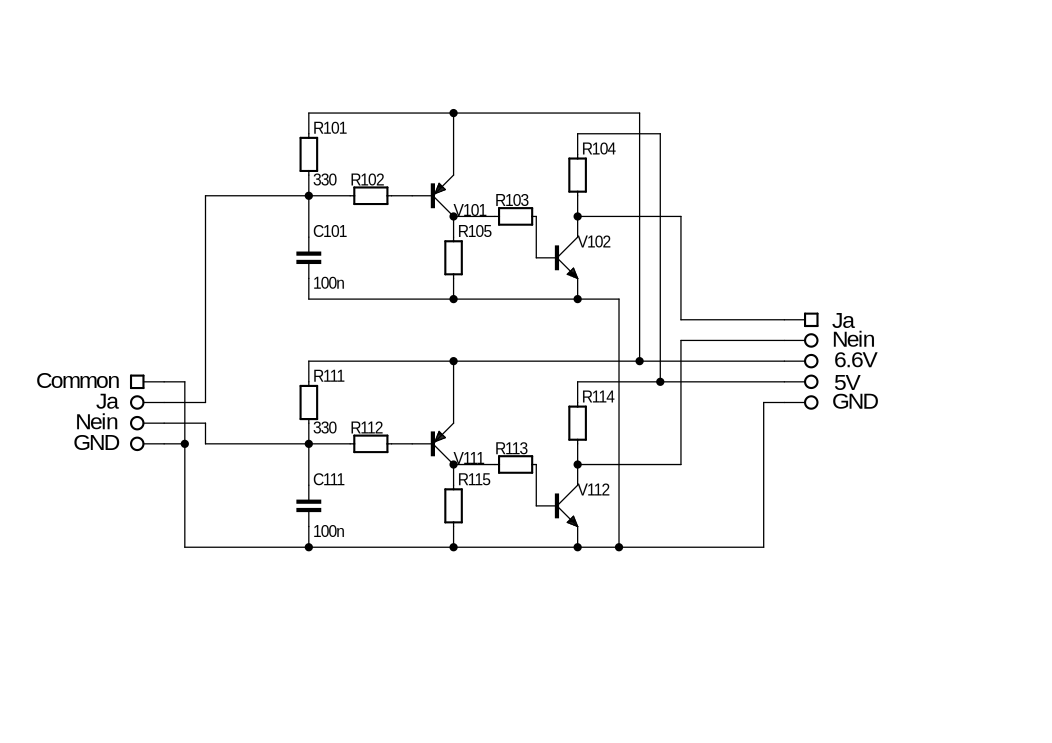
\includegraphics[scale=\schscale]{fig/xlr_pegelwandler_v_1_2_sch.pdf}
	\caption{Schema}
	\label{sch:pegw}
\end{figure}

\subsection{Funktion}
Die beiden Kanäle sind identisch aufgebaut. Nachfolgend wird die Funktionsweise anhand der Teilschaltung 10x gezeigt. R101 fungiert als Pull-Up Widerstand. Um Störungen durch das lange Kabel des an CON101 angeschlossenen Tasters zu verringern ist dieser relativ niederohmig ausgeführt. C101 filtert hochfrequente Störungen und stellt einen gewissen Schutz der Basis von V101 gegen ESD dar. V101 und V102 arbeiten als Schalter in Emitterschaltung. Im Ruhezustand sperren beide Transistoren. Das Ausgangssignal ist HIGH. Wird der Taster gedrückt, sinkt die Spannung am Eingang der Schaltung. Dadurch wird V101 leitend die Spannung am Kollektor von V101 steigt. Dies bewirkt, dass V102 letitend wird und die Ausgangsspannung LOW wird. Beim Loslassen des Tasters kehrt die Schaltung in ihren Ursprungszustand zurück. 

\subsubsection{Dimensionierung}
\[ \begin{array}{l}
R101 = \frac{U_B}{I_{sw}}\\
U_B = 6.6 V\\
I_{sw} = 20 mA\\
\Rightarrow R101 = \frac{6.6V}{20mA} = \underline{\underline{330 \Omega}}
\end{array} \]
\[ \begin{array}{l}
P_{R101} = \frac{{U_{R101}}^2}{R101} = \frac{{U_{Bat_{max}}}^2}{R101} = \frac{7.2 V}{330 \Omega} = 157 mW
\end{array} \]
%
\[ \begin{array}{l}
R104 = \frac{5 V - U_{O_H}}{I_O} = \frac{5 V - 4.? V}{0.5 mA} = 
\end{array} \]

\subsection{Layout}
\begin{figure}[h!]
	\centering
	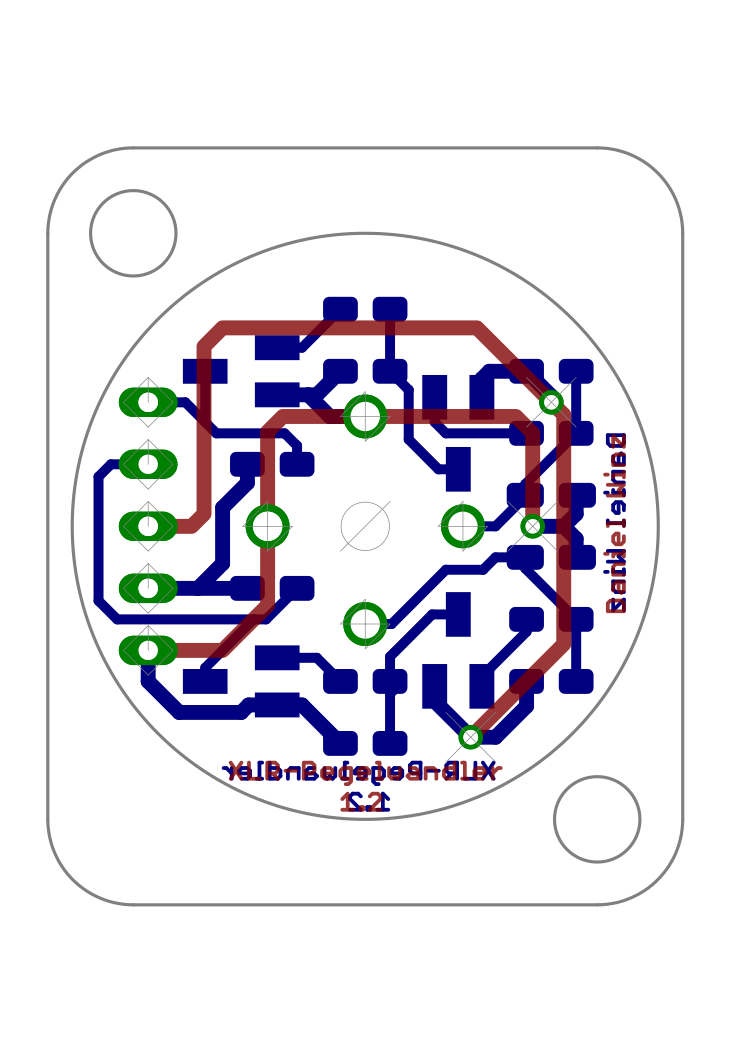
\includegraphics[scale=\layscale]{fig/xlr_pegelwandler_v_1_2_lay_transp.pdf}
	\caption{Layout}
	\label{lay:pegw}
\end{figure}
